\documentclass{llncs}
%\usepackage{acl2015}
\usepackage{times}
\usepackage{booktabs}
\usepackage{latexsym}
\usepackage{graphicx}
\usepackage{array,etoolbox}
\usepackage{tikz}
\usepackage{makecell}
\renewcommand{\floatpagefraction}{.8}
\preto\tabular{\setcounter{magicrownumbers}{0}}
%\newcommand{\circlednumber}[1]{\raisebox{.5pt}{\textcircled{\raisebox{-.9pt} {#1}}}}
\newcommand*\circlednumber[1]{\tikz[baseline=(char.base)]{
    \node[shape=circle,draw,inner sep=1pt, minimum size=1pt] (char) {\footnotesize{#1}};}}
\newcounter{magicrownumbers}
\def\rownumber{}
%\setlength\titlebox{5cm}
\newcommand\mlex{M^{\scriptscriptstyle LEX}}
\newcommand\msyn{M^{\scriptscriptstyle SYN}}
\newcommand\mstd{M^{\scriptscriptstyle STD}}
\newcommand\slex{S^{\scriptscriptstyle LEX}}
\newcommand\ssyn{S^{\scriptscriptstyle SYN}}
\newcommand\sstd{S^{\scriptscriptstyle STD}}
% You can expand the titlebox if you need extra space
% to show all the authors. Please do not make the titlebox
% smaller than 5cm (the original size); we will check this
% in the camera-ready version and ask you to change it back.


\title{Fusion Techniques for Named Entity Recognition and Word Sense Induction and Disambiguation}

\author{Edmundo-Pavel Soriano-Morales \and Julien Ah-Pine\
 \and Sabine Loudcher}
%
%\authorrunning{Ivar Ekeland et al.} % abbreviated author list (for running head)
%
%%%% list of authors for the TOC (use if author list has to be modified)
%\tocauthor{Ivar Ekeland, Roger Temam, Jeffrey Dean, David Grove,
%Craig Chambers, Kim B. Bruce, and Elisa Bertino}
%
\institute{University of Lyon, Universit\`{e} Lyon 2, Laboratoire ERIC, Lyon, France,\\
\email{\{edmundo.soriano-morales, julien.ah-pine, sabine.loudcher\}@univ-lyon2.fr}}
\date{}

\begin{document}
\maketitle
\begin{abstract}
In this paper we explore the use of well-known multimodal fusion techniques to solve two prominent Natural Language Processing tasks. Specifically, we focus on solving Named Entity Recognition and Word Sense Induction and Disambiguation by applying feature-combination methods that have already shown their efficiency in the multimedia analysis domain. We present a series of experiments employing fusion techniques in order to combine textual linguistic features. Our intuition is that by combining different types of features we may find semantic relatedness among words at different levels and thus, the combination (and recombination) of these levels may yield gains in terms of metrics' performance. To our knowledge, employing these techniques has not been studied for the tasks we address in this paper. 
We test the proposed fusion techniques on three datasets for named entity recognition and one for word sense disambiguation and induction. Our results show that the combination of textual features indeed improves the performance compared to single feature representation and the trivial feature concatenation.
\end{abstract}


\section{Introduction}

Named Entity Recognition (NER) and Word Sense Induction and Disambiguation (WSI/ \allowbreak WSD) requires textual features to represent the similarities between words in order to discern between different words' meanings. NER goal is to automatically discover, within a text, mentions that belong to a well-defined semantic category. The classic task of NER involves detecting entities of type Location, Organization, Person and Miscellaneous. The task is of great importance for more complex NLP systems, e.g, relation extraction, opinion mining. Common solutions to NER consist on one of the following: via matching patterns created manually or extracted semi-automatically; or by training a supervised machine learning algorithm with large quantities of annotated text. The latter being the currently more popular solution to this task.




%In the classic case of NER, we need to determine, given its context, whether a word is referring a person, a location, an organization or another miscellaneous entity. On the other hand, in WSI/WSD the goal is to determine and assign the specific meaning of a target word, again based on its context.

Word Sense Induction and Disambiguation involves two closely related tasks\footnote{Even though these tasks are related, they are independent from one another. Still, in this paper we consider them to be a single one.}. WSI aims to automatically discover the set of possible senses for a target word given a text corpus containing several occurrences of said target word. Meanwhile, WSD takes a set of possible senses and determines the most appropriate sense for each instance of the target word according to the instance's context. WSI is usually approached as an unsupervised learning task, i.e., a cluster method is applied to the words occurring in the instances of a target word. The groups found are interpreted as the senses of the target word. The WSD task is usually solved with knowledge-based approaches, based on WordNet; or more recently with supervised models which require annotated data.

As stated before, both tasks rely on features extracted from text. Usually, these representations are obtained from the surrounding context of the words in the  input corpus. Mainly  two types of representations are used. According to their nature we call these features lexical and syntactical. 	The first type requires no extra information than that contained already in the analyzed text itself. It consists merely on the tokens surrounding a word, i.e., those tokens that come before and after within a fixed window. The second type, syntactical features, is similar to the lexical representation in that we also consider as features the tokens that appear next to the corpus' words. Nonetheless, it requires a deeper degree of language understanding. In particular, these features are based on part of speech tags, phrase constituents information, and syntactical functionality between words, portrayed by syntactical dependencies. Likewise, specific features, particular to a task are also employed. These features later on become standard features in the literature.

%For example, in NER, some standard features used in the literature include whether a word begins with an upper-case letter, the type of prefix and suffix of the word itself as well as the context words, and so on.

%In the latter case, as with any supervised model, we need to first define a set of features that will better represent each token. In this work, we make use of three different types of linguistic data, that is, (1) lexical co-occurrence, (2) grammatical dependency relations and (3) constituent-tree branch membership to try and solve the NER task. More importantly, we propose a fusion framework that uses different methods to combine these three sources of information (among others) into a single representation model.

Most of the approaches in the literature dealing with these tasks use each of these features independently or stacked together, i.e., different feature columns in an input representation space matrix. In the latter case, features are usually combined without regards to their nature. 

The main intuition of the present work is that word similarities may be found at different levels according to the type of features employed. In order to exploit these similarities, we look into multimedia fusion methods.  In order to better perform an analysis task, these techniques combine multimodal representations, their corresponding similarities, or the decisions coming from models fitted with these features. In this paper, we try to mutually complement independent representations by utilizing said fusion techniques to combine (or fuse) features in the hope of improving the performance of the tasks at hand, specially compared to the use of features independently. 

Fusion techniques have previously shown their efficiency, mainly on text and image related tasks, where there is a need to model the relation  between images and text extracts.
%
%. 
%
Here, in order to apply multimedia fusion techniques, we consider textual features as different modalities, i.e., instead of having textual and image features we have lexical and syntactical features. The main contribution of this work is to assess the effectiveness of simple yet untested techniques to combine classical and easy to obtain textual features. As a second contribution, we propose a series of feature combination and recombination to attain better results. We test our intuitions on both NER and WSI/WSD tasks and over four different corpora: CoNLL-2003 \cite{SangM03}, WikiNER and Wikigold \cite{Balasuriya2009} for NER; Semeval-2007 \cite{Agirre2007} for WSI/WSD.

The rest of the paper is organized as follows: in Section 2, we go into further details about fusion techniques. 
%as well as its application in the NLP domain. 
We introduce the fusion operators that we use in our experiments in Section 3. Then, in Section 4 we show the effectiveness of the presented methods by testing them on NER and WSI/WSD and their respective datasets. Finally, in Section 5 we present our conclusions and future directions to explore.

\section{Background and Related Work}
 
In this section, we first describe the fusion techniques we use in our methodology as well as relevant use-cases where they have been employed. We then briefly                                                
\subsection{Multimodal Fusion Techniques}
Multimodal fusion is a set of popular techniques used in multimedia analysis tasks. These methods integrate multiple media features, the affinities among these attributes or the decisions obtained from systems trained with said features, to obtain rich insights about the data being used and thus to solve a given analysis  task \cite{Ah-PineCC15,AtreyHEK10}. We note that these techniques come at the price of augmenting the training time of a system by increasing both the dimension space and/or the sparsity of a given feature matrix.


In the multimodal fusion literature we can discern two main common types of techniques: early fusion and late fusion. 
\subsubsection{Early Fusion}
This technique is the most widely used fusion method. The principle is simple: we take both modal features and concatenate them into a single representation matrix. More formally, we consider two matrices  that represent different modality features each  over the same set of individuals. To perform early fusion we concatenate them column-wise, such that we form a new matrix having the same number of lines but increasing the number of columns to the sum of the number of columns of both matrices. The matrices may also be weighted as to control the influence of each modality.

The main advantage of early fusion is that a single unique model is fitted while leveraging the correlations among the concatenated features. The method is also easy to integrate into an analysis system. The main drawback is that we increase the representation space and may make it harder to fit models over it.
%

%   of shape $(n, m + p)$. Following the literature notation of [vulic], the early fusion representation matrix EF is defined as:
%\begin{equation}
%EF = \alpha \times X_1 || (1 - \alpha) \times X_2
%\end{equation}

%where $||$ represents the column-wise concatenation operation and α is the parameter that determines the contribution of each modality. 
%
%Early fusion has been employed in several multimodal tasks. For example, [?]. 
\subsubsection{Late Fusion}
In contrast to early fusion, in late fusion the combination of multimodal features are generally performed at the decision level, i.e., using the output of independent models trained  each with an unique set of features \cite{ClinchantAC11}. In this setting,  decisions produced by each model are combined into a single final result set.
%
The methods used to combine preliminary decisions usually involve one of two types: rule-based (where modalities are combined according to domain-specific knowledge) or linear fusion (e.g., weighting and then adding or multiplying both matrices together). This type of fusion is very close to the so-called ensemble methods in the machine learning literature.
%
Late fusion combines both modalities in the same semantic space. In that sense,  we may also combine modalities via an affinity representation instead of final decision sets. In other words, we can combine two modality matrices by means of their respective similarities. A final representation is then usually obtained by adding the weighted similarity matrices.
%

The advantages of late fusion include the combination of features at the same level of representation (either the fusion of decisions or similarity matrices). Also, given that independent models are trained separately, we can chose which algorithm is more adequate for each type of
features.

%For example, in information retrieval (Ah-Pine et al., 2015), lexicon learning (Vulic et al., 2016), coreference resolution (Eisenstein and Davis, 2007); different types of representations (different modalities) can be combined in order to take advantage of the complementarity existing among them
\subsubsection{Cross-media Similarity Fusion}
%
A third type of fusion technique, cross-media similarity fusion (or simply cross fusion),   introduced in \cite{Ah-PineCC15,ClinchantAC11}, is defined and employed to propagate a single similarity matrix into a second similarity matrix. In their paper, the authors propagated information from textual media towards visual media. In our case, we transfer information among textual features. For example, to perform a cross fusion between lexical and syntactical features, we perform the following steps: 
\begin{enumerate}
\item Compute the corresponding similarity matrices for each type of feature.
\item Select only the $k$-nearest neighbor for each word within the lexical similarity matrix. These neighbors are to be used as lexical representatives to enrich the syntactical similarities.
\item Linearly combine both similarity matrices (lexical $k$-nearest lexical neighbors with the syntactical features) via a matrix product.
\end{enumerate}  

Cross fusion aims to bridge the semantic gap between two modalities by using the most similar neighbors as proxies to transfer valuable information  from one modality onto another one. Usually, the result of a cross fusion is combined with the previous techniques, early and late fusion. In this paper we perform  experiment in that sense.

\subsubsection{Hybrid Fusion}
We may leverage the advantages of the previous two types of fusion techniques by combining them once more in a hybrid setting. As described in \cite{AtreyHEK10,yu2014informedia}, the main idea is to simultaneously combine features at the feature level, i.e., early fusion, and at the same semantic space or decision level. Nonetheless, they define a specific type of hybrid fusion. In this paper, we adopt a looser definition of hybrid fusion. That is, we perform hybrid fusion by leveraging the combination of the fusion strategies described before.

We consider the first three types of fusion techniques (early fusion, late fusion and cross fusion) as the building blocks to the experiments we conduct.  While we work with a single modality, i.e., textual data, we consider the different kinds of features extracted from it as distinct modalities. Our intuition being that the semantic similarities among words in these different spaces can be combined in order to exploit the latent complementarity between the lexical and syntactical representations. The fusion should therefore improve the performance of the NLP tasks at hand, NER and WSI/WSD.

Our first goal is to assess the effectiveness of the classic fusion methods and then, as a second goal, to propose new combinations that yield better outcomes in terms of performance than the simpler approaches. The new combinations are found empirically. Nonetheless, as we will show, their effectiveness replicates across different datasets and NLP tasks. 
%In a general sense,
%having two similarity matrices $S_1$ and $S_2$ defined as above, we define the cross-media similarity fusion as:
%
%\begin{equation}
%XF = \mathbf{K}(S_1, k) \cdot S_2
%\end{equation}
%
%where $\mathbf{K}$ is a row-wise function that keeps only the top-k values of the similarity matrix S 1 and
%assigns zero to the rest of the line.

%In Table [] we show a synthetic table with the literature works on fusion cited in this section. We present the task solved by each contribution, the type of fusion used, the modalities involved and finally the performance gain obtained while using the fusion techniques.

\subsection{NER and WSI/WSD}
To the best of our knowledge, there is no work that addresses both NER and WSI/WSD explicitly while using fusion techniques from the multimedia analysis domain. Still, we base our experiments on those carried on in \cite{Collins2002,Daume2006,GoyalH14} using well-known supervised (structured perceptron) and unsupervised (spectral clustering) learning algorithms. A thorough review on NER and WSI/WSD can be found in \cite{nadeau2007survey} and \cite{navigli2009word}, respectively.

\section{Methodology}
In the present section we address the core of the work performed in this paper.
We formally describe the fusion techniques we employ in the next section. Also, we  delineate the procedure followed in our experiments. 


%This kind of fusion combinations is somewhat similar to previously employed approaches which join early fusion with cross fusion operators to construct random-walk based fusion methods \cite{Ah-PineCC15,GialampoukidisM16}. These techniques iterate over the fusion operators several times in the hopes of better propagating useful information across modalities. Still, we do not perform any kind of iteration. Our approaches perform a single step to obtain a representation matrix.



\begin{figure*}[t]
\centering

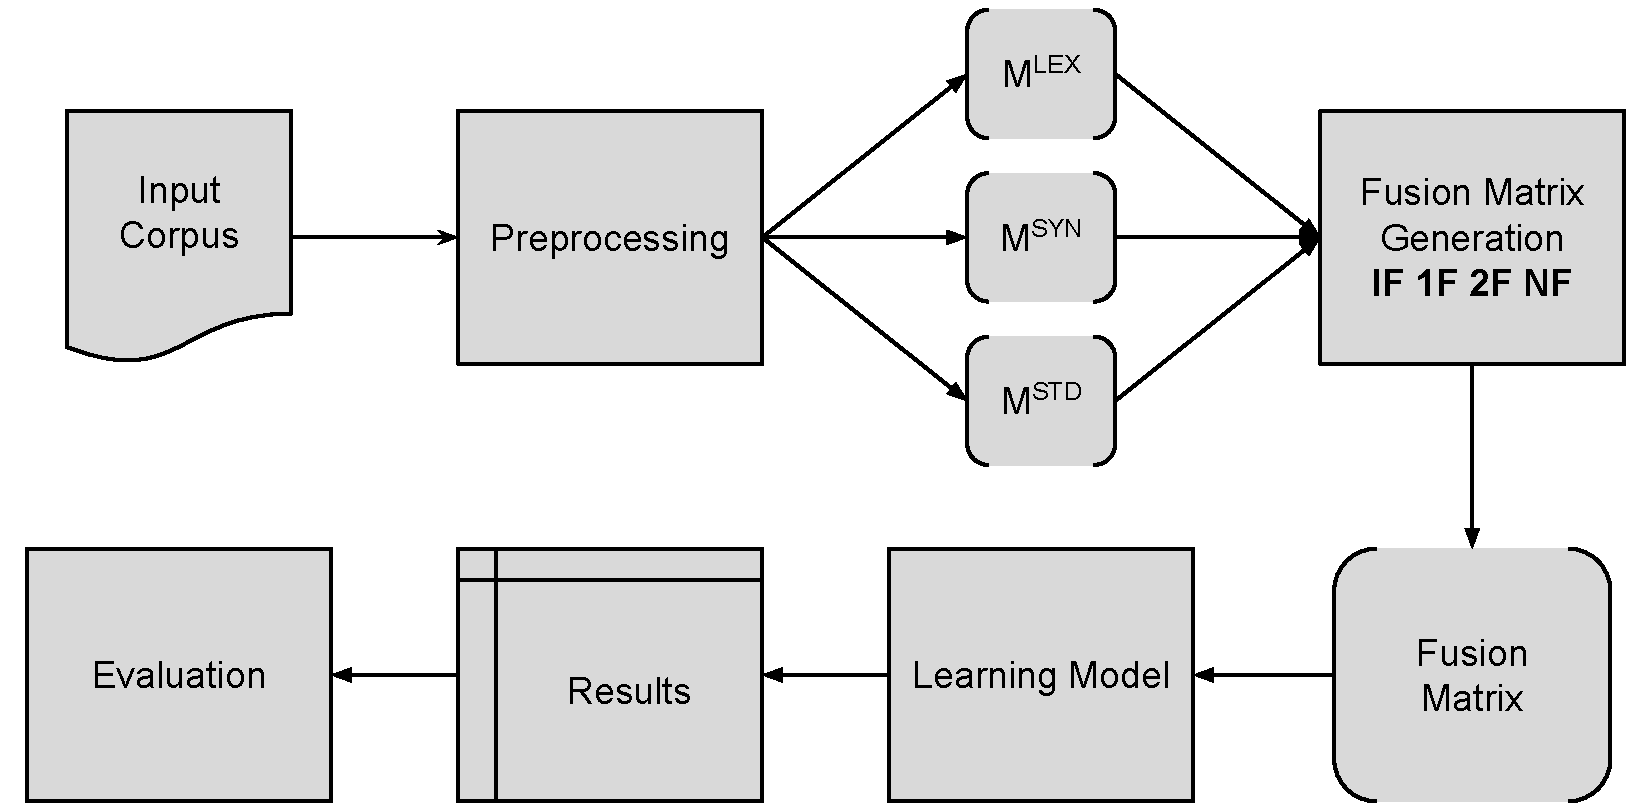
\includegraphics[width=0.85\linewidth]{img/diag_metodo}
\caption{Steps followed on our experiments. First the corpus is preprocessed, then features are extracted from the text. A fusion matrix is generated, which in turn is used as input to a learning algorithm. Finally, the system yields its results and to be analyzed.}
\label{fig:diagmetodo}
\end{figure*}

The experiments we carry on consist in generating fusion matrices that will serve as input to a learning algorithm in order to solve NER and WSI/WSD. These input feature matrices are based upon lexical, syntactical, or other types of representation. The procedure can be seen in Figure \ref{fig:diagmetodo}.

\subsection{Fusion Strategies}
We begin by presenting a  formal definition of the fusion techniques employed and described in the previous sections. We define (weighted) early fusion, late fusion and cross fusion as follows:
\paragraph{Early Fusion}
\begin{equation}
E(A,B) = \mathbf{hstack}(A , B)
\end{equation}
\paragraph{Weighted Early Fusion}
\begin{equation}
wE_\alpha(A,B) = \mathbf{hstack}(\alpha\cdot A , (1-\alpha)\cdot B)
\end{equation}
\paragraph{Late Fusion}
\begin{equation} \label{eq:late-fusion}
L_\beta(A,B) = \beta \cdot A + (1 - \beta)\cdot B
\end{equation}
\paragraph{Cross fusion}
\begin{equation}
X_{\gamma}(A,B) = \mathbf{K}(A,\gamma) \times B
\end{equation}

%\vspace{.3cm}

Parameters $A$ and $B$ are arbitrary input matrices. They may initially represent, for example,  the lexical ($M^{LEX}$) or syntactical based ($M^{SYN}$) features matrix, or their  corresponding similarity matrices, $S^{LEX}$ and  $S^{SYN}$, ~respectively. In a broader sense, matrices $A$ and $B$ may represent any pair of valid\footnote{Valid in terms of having compatible shapes while computing a matrix sum or multiplication.} fusion matrices. 

In early fusion, $E(A,B)$, the matrices $A$ and $B$ are combined together via a  function called $\mathbf{hstack}$ which concatenates, column-wise, both matrices $A$ and  $B$. Weighted early fusion  represents the same operation as before with an extra parameter: $\alpha$, which controls the relative importance of each matrix. In the following, we refer to both operations as early fusion. When $\alpha$ is determined, we refer to weighted early fusion.

Regarding late fusion $L_\beta(A,B)$, the  $\beta$ parameter determines again the importance of the  matrix $A$,  and consequently also the relevance of matrix $B$.

In cross fusion $X_\gamma(A,B)$, the $\mathbf{K}(\cdot)$ function keeps the top-$\gamma$ closest words (columns) to each word (lines) while the rest of the values are set to zero. 

Using the previously defined operators, we distinguish four levels of experiments: 
\begin{enumerate}
\item \textbf{Single Features}: in this phase we consider the modalities independently as input to the learning methods. For instance, we may train a model for NER using only the lexical features matrix $M^{LEX}$.
\item \textbf{First Degree Fusion}: we  consider the  three elementary fusion techniques by themselves (early fusion, late fusion, cross fusion) without any recombination.  These experiments, as well as those from the previous level, serve as the baselines we set to surpass in order to show the efficacy of the rest of the fusion approaches.
As an example, we may obtain a representation matrix by performing an early fusion between the lexical matrix and the syntactical features matrix: $E(M^{LEX}, M^{SYN})$. In this level we distinguish two types of cross fusion: Cross Early Fusion (XEF) and Cross Late Fusion (XLF). The first one combines a similarity matrix with a feature matrix: $X(\slex, \msyn)$. The second one joins a similarity matrix with a similarity matrix: $X(\ssyn, \slex)$.
\item \textbf{Second Degree Fusion}:  we recombine the outputs of the previous two levels with the elementary techniques. This procedure then yields a recombination of "second-degree" among fusion methods. We introduce the four types of second degree fusions in the following list. Each one is illustrated with an example:

\begin{enumerate}
\item Cross Late Early Fusion (XLEF): $X(X(\sstd, \ssyn), \mstd)$
\item Cross Early Early Fusion (XEEF: $X(\sstd, X(\sstd, \ssyn))$
\item Early Cross Early Fusion (EXEF): $E(\mstd,X(\slex, \mstd))$
\item Late Cross Early Fusion (LXEF): $L(\mstd, X(\sstd, \mstd))$
\end{enumerate}

% A second-degree fusion would be an early fusion of the lexical feature matrix with a cross fusion, expressed as $E(M^{LEX}, \allowbreak X(S^{STD}, M^{STD}))$.   
\item \textbf{N-Degree Fusion}: in this last level we follow a similar approach to the previous level by combining the output of the second-degree fusion level multiple times (more than two times) with other second-degree fusion outputs. 
Again, in this level we test the following two fusion operations:
\begin{enumerate}
\item Early Late Cross Early Fusion (ELXEF): $E(\mstd, L(\mstd, X(\sstd, \mstd)))$
\item Early ELXEF (EELXEF): $E(\mlex, E(E(\mstd,  L(\mstd, X(\sstd, \mstd))),\allowbreak L(\mlex, X(\ssyn, \mlex))))$
\end{enumerate}

%As an example, the equation $E(L(M^{STD}, \allowbreak X(S^{STD}, M^{STD})),  L(M^{LEX}, X(S^{SYN}, M^{LEX})))$  \allowbreak denotes the early fusion between two operations: (1) a late fusion between a lexical-features matrix and a cross fusion, and (2),  another late fusion consisting of a standard-features matrix (this matrix is detailed below)  and a cross fusion. In general, we determine a n-degree fusion empirically. That is to say, we look at the performance of second-degree fusions and try to improve the performance of the systems by recombining the fusion outputs via a n-degree combination. This process is in fact applied during the second-degree fusions also. 
	\end{enumerate}   
\subsection{Feature Matrices}
In the previous subsection we presented the fusion operators used in our experiments. Below we detail the three types of features used to describe the words of each of the tested corpus.
\subsubsection{Lexical Matrix (LEX)}
For each token in the corpus, we use a lexical window of two words to the left and two words to the right, plus the token itself. Specifically, for a target word $w$, its lexical context is $(w_{-2}, w_{-2}, w, w_{+1}, w_{+2})$. This type of context features is typical for most systems studying the surroundings of a word, i.e., using a distributional approach \cite{LevyG14}.
% We retake the example phrase from \cite{LevyG14}, the lexical-based features of the phrase \textit{Australian scientist discovers start with telescope}, are shown in Table \ref{tab:lex-contexts}.
%\begin{table*}[ht]
%\centering
%\begin{tabular}{ll}
%\hline 
% \textbf{Word} & \textbf{Features} \\ 
%\hline 
%Australian & word:Australian, word+1:scientist, word+2:discovers\\ 
%scientist  &  word-1:Australian, word:scientist, word+1:discovers, word+2:star\\ 
%discovers & word-2:Australian, word-1:scientist, $\dots$, word+2:telescope \\ 
%star & word-2:scientist, word-1:discovers, word:star, $\dots$, word+2:telescope \\ 
%with & word-2:discovers, word-1:star, word:with, word+1:telescope \\ 
%telescope  &  word-2:star, word-1:with, word:telescope \\ 
%\hline \
%\end{tabular} 
%\label{tab:lex-contexts}
%\caption{Lexical features corresponding to the phrase \textit{Australian scientist discovers start with telescope}.}
%\end{table*} 

\subsubsection{Syntactical Matrix (SYN)}
Based on the syntactic features used in   \cite{LevyG14,Panchenko2017}, we derive contexts based on the syntactic relations a word participates in, as well as including the part of speech (PoS) of the arguments of these relations. Formally, for a word $w$ with modifiers $m_1, \dots, m_k$ and their corresponding PoS tags $p^m_1, \dots, p^m_k$; a head $h$ and its corresponding PoS tag $p_h$, we consider the context features $(m_1, p_{m_1}, lbl_1), \dots, \allowbreak (m_k, p_{m_k}, lbl_k), \allowbreak (h,p_h,lbl\_inv_h)$. In this case, $lbl$ and $lbl_{inv}$ indicate the label of the dependency relation and its inverse, correspondingly. Using syntactic dependencies as features should yield more specific similarities, closer to synonymy, instead of the broader topical similarity found through lexical contexts.
%For the phrase \textit{Australian scientist discovers start with telescope} the dependency-based context is shown in Table \ref{tab:syn-contexts}.
\subsubsection{NER Standard Features Matrix (STD)}
The features used for NER are based on those used in \cite{Daume2006,Balasuriya2009}. The feature set consists of: the word itself, whether the word begins with capital letter, prefix and suffix up to three characters (within a window of two words to the left and two words to the right), and the PoS tag of the current word. These features are considered to be standard in the literature. We note that the matrix generated with these features is exclusively used in the experiments regarding NER.	

\subsection{Learning Methods}
We use supervised and unsupervised learning methods for NER and WSI/WSD respectively. On the one hand, for NER, as supervised algorithm, we use an averaged structured perceptron \cite{Collins2002,Daume2006} to determine the tags of the named entities. We considered Logistic Regression and linear SVM. We chose the perceptron because of its performance and its lower training time.

On the other hand, for WSD/WSI, specifically for the induction part, we applied spectral clustering, as in  \cite{GoyalH14}, on the input matrices in order to automatically discover senses (a cluster is considered a sense). Regarding disambiguation, we trivially assign senses to the target word instances according to the number of common words in each cluster and the context words of the target word. In other words, for each test instance of a target word, we select the cluster (sense) with the maximum number of shared words with the current instance context.


%\begin{table*}
%\centering
%\begin{tabular}{ll}
%\hline 
% Word & Contexts \\ 
%\hline 
%Australian & scientist/NN/amod\_inv \\ 
%scientist  &  Australian/JJ/amod, discovers/VBZ/nsubj\_inv\\ 
%discovers & scientist/NN/nsubj, star/NN/dobj, telescope/NN/nmod:with \\ 
%star & discovers/VBZ/dobj\_inv \\ 
%telescope  &  discovers/VBZ/nmod:with\_inv \\ 
%\hline \
%\end{tabular} 
%\label{tab:syn-contexts}
%\caption{Syntactic contexts corresponding to the phrase \textit{Australian scientist discovers start with telescope}.}
%\end{table*}




\section{Experiments and Evaluation}


We experiment with four levels of fusion: Single Features (SF), First-degree Fusion (1F), Second-degree Fusion (2F) and N-degree Fusion (NF). The representation matrices for NER come from lexical context features $M^{LEX}$, syntactical context features $M^{SYN}$ or standard features $M^{STD}$.  On the other hand, experiments on WSI/WSD exclusively employ matrices $M^{LEX}$ and $M^{SYN}$.

Our first goal is to compare the efficiency of the basic multimedia fusion techniques applied to  single-modality multi-feature NLP tasks, namely NER and WSI/WSD. A second goal is to empirically determine a fusion combination setting able to leverage the complementarity of our features.

To this end, we evaluate the aforementioned 4 fusion levels. We note that the fusion combinations in the third and fourth level (2F and NF) are proposed based on the results obtained in the previous levels. In other words, in order to reduce the number of experiments, we restrict our tests to the best performing configurations. This is due to the large number of possible combinations (an argument to a fusion operation may be any valid output of a second fusion operation).


\subsection{Named Entity Recognition}

\subsubsection{Pre-processing}

As is usual when preprocessing text before performing named entity recognition, \cite{RatinovR09}, we normalize tokens that include numbers. 
%For example, the token 1980 becomes *DDDD* and 212-325-4751 becomes *DDD*-*DDD*-*DDDD* . T
This allows a degree of abstraction to tokens that contain years, phone numbers, etc. 
%We do not normalize punctuation marks.

\subsubsection{Features}
The linguistic information we use are extracted with the Stanford's CoreNLP parser \cite{manning2014}. Again, the features used for these experiments on NER are those described before: lexical, syntactic and standard features, i.e., $M^{LEX}$, $M^{SYN}$, and $M^{STD}$, respectively. 

\subsubsection{Test Datasets}We work with three corpora coming from two different domains:
\begin{itemize}
\item [(1)] CoNLL-2003 (CONLL): This dataset was used in the language-independent named entity recognition CoNLL-2003 shared task \cite{SangM03}. It contains selected news-wire articles from the Reuters Corpus. Each article is annotated manually. It is divided in three parts:  training (\textit{train}) and two testing sets (\textit{testa} and \textit{testb}). The training part contains 219,554 lines, while the test sets contain 55,044 and 50,350 lines, respectively. The task was evaluated on the \textit{testb} file, as in the original task.
\item [(2)]WikiNER (WNER): A more recent dataset \cite{Balasuriya2009} of selected English \allowbreak Wikipedia articles, all of them annotated automatically with the author's semi-supervised \allowbreak method. In total, it contains 3,656,439 words. 
\item[(3)] Wikigold (WGLD): Also a corpus of Wikipedia articles, from the same authors of the previous corpus. Nonetheless, this was annotated manually. This dataset is the smaller, with 41,011 words. We used this corpus to validate human-tagged Wikipedia text. These three datasets are tagged with the same four types of entities: Location, Organization, Person and Miscellaneous.

%Otherwise, while it is faster to train models with this corpus, it may be the case that they are not able to properly fit the data given its size, and thus performance is lower than the other datasets.

\end{itemize}
%
\subsubsection{Evaluation Measures}
We evaluate our NER models following the standard CoNLL-2003 evaluation script. Given the amount of experiments we carried on, and the size constraints, we report exclusively the total F-measure for the four types of entities (Location, Organization, Person, Miscellaneous). WNER and WGLD datasets are evaluated on a 5-fold cross validation.

\subsubsection{Results}
We present in this subsection the results obtained in the named entity recognition task, while employing the 4 levels of fusion proposed in the previous section.

In contrast to other related fusion works \cite{Ah-PineCC15,ClinchantAC11,GialampoukidisM16}, we do not focus our analysis on the impact of the parameters of the fusion operators. Instead, we focus our analysis on the effect of the type of linguistic data being used and how, by transferring information from one feature type to another, they can be experimentally recombined to generate more complete representations.

Regarding the fusion operators' parameters, we empirically found the best configuration for $\beta$, from late fusion $L_\beta(A,B) = \beta \cdot A + (1 - \beta)\cdot B$, is $\beta=0.5$. This implies that an equal combination is the best linear fusion for two different types of features.

In respect of the $\gamma$ parameter, used in cross fusion $X_{\gamma}(A,B) = \mathbf{K}(A,\gamma) \times B$, we set $\gamma=5$. This indicates that just few high quality similarities attain better results than utilizing a larger quantity of lower quality similarities.

\begin{table}[!tbp]
\centering
\caption{NER F-measure results using the Single Features over the three datasets. These values serve as a first set of baselines. }
\label{tab:ner-blines}
\begin{tabular}{@{}lccc@{}}
\toprule
$A$                           & \multicolumn{3}{c}{\textbf{Single Features}} \\ \midrule
                & \textbf{CONLL}    & \textbf{WNER}     & \textbf{WGLD}    \\ \cmidrule{2-4}
$M^{\scriptscriptstyle STD}$                        & 77.41    & 77.50    & 59.66   \\
$M^{\scriptscriptstyle LEX}$                       & 69.40    & 69.17    & 52.34   \\
$M^{\scriptscriptstyle SYN}$                        & 32.95    & 28.47    & 25.49   \\ \bottomrule
\end{tabular}

\end{table}
\paragraph{Single Features}
Looking at Table \ref{tab:ner-blines}, we see that the best independent features, in terms of F-measure come from the standard representation matrix $\mstd$. This is not surprising as these features, simple as they may be, have been used and proved extensively in the NER community. On the other hand, $\mlex$ performs relatively well, considering it only includes information contained in the dataset itself. Nevertheless, this representation that this kind of lexical context features are the foundation of most word embedding techniques used nowadays.
While we expected better results from the syntactical features $\msyn$, as they are able to provide not only general word similarity, but also functional, getting close to synonymy-level \cite{LevyG14},  we believe that the relatively small size of the datasets do not provide enough information to generalize 
\paragraph{First Degree Fusion }
In Table \ref{tab:ner-1d} we present the First Degree fusion level. The best performance is obtained by trivially concatenating the representation matrices. This baseline proved to be the toughest result to beat. Late fusion does not perform well in this setting, still, we see further on that by linearly combining weighted representation matrices, we can add information to an already strong representation. Finally, regarding the cross fusion techniques, cross early and late fusion, we see that they depend directly on the information contained in the similarity matrices. We note that, as is the case on single features, the combinations with matrix $\sstd$ yield almost always the best results. While these fusion techniques by themselves may not offer the best results, we see below that by recombining them with other types of fusion we can improve the general performance of a representation.




\begin{table}[!tb]
\centering
\setlength\tabcolsep{2pt}
\begin{minipage}[t]{0.48\textwidth}
\centering

\caption{NER F-measure results using first degree fusion (1F). $B$ is either indicated on the table or specified as follows. Looking at EF,  $\hat{b}_{EF} = E(\msyn, \mstd)$. In XEF, ${b}^*_{\scriptscriptstyle XEF}$ takes the matrix from the set $\{M^{\scriptscriptstyle LEX}, M^{\scriptscriptstyle STD} \}$ which yields the best performing result. In XLF, $\hat{b}_{\scriptscriptstyle XLF}^{*}$ corresponds to the best performing matrix in $\{S^{\scriptscriptstyle LEX},S^{\scriptscriptstyle SYN}\}$. These configurations serve as the main set of baseline results.}
\label{tab:ner-1d}
\centering
%\tablewidth=\textwidth
\begin{tabular}{@{}llccc@{}}
\toprule
    $A$      &    $B$       & \multicolumn{3}{r}{\textbf{Early Fusion} }                                            \\ \midrule
          &           & \textbf{CONLL}                      & \textbf{WNER}                      & \textbf{WGLD}                      \\ \cmidrule{3-5}
$M^{\scriptscriptstyle LEX}$ & $M^{\scriptscriptstyle SYN}$ & 72.01                      & 70.59                     & 59.38                     \\
$M^{\scriptscriptstyle LEX}$ & $M^{\scriptscriptstyle STD}$ & 78.13                      & 79.78                     & 61.96                     \\
$M^{\scriptscriptstyle SYN}$ & $M^{\scriptscriptstyle STD}$ & 77.70                      & 78.10                     & 60.93                     \\
$M^{\scriptscriptstyle LEX}$ & $\hat{b}_{EF}$ & \textbf{78.90}                      & \textbf{80.04}                     & \textbf{63.20}                     \\
\midrule
          &           & \multicolumn{3}{r}{\textbf{Late Fusion} }                                             \\
\midrule     
          &           & \textbf{CONLL}                      & \textbf{WNER}                      & \textbf{WGLD}                      \\ \cmidrule{3-5}
$S^{\scriptscriptstyle LEX}$ & $S^{\scriptscriptstyle SYN}$ & \textbf{61.65}                      & 58.79                     & 44.29                     \\
$S^{\scriptscriptstyle LEX}$ & $S^{\scriptscriptstyle STD}$ & 55.64                      & \textbf{67.70}                     & 48.00                     \\
$S^{\scriptscriptstyle SYN}$ & $S^{\scriptscriptstyle STD}$ & 50.21                      & 58.41                     & \textbf{49.81}                     \\
\midrule
          &           & \multicolumn{3}{r}{\textbf{Cross Early Fusion}} \\
\midrule
          &           & \textbf{CONLL}                      & \textbf{WNER}                      & \textbf{WGLD}                      \\ \cmidrule{3-5}
$S^{\scriptscriptstyle LEX}$ &$M^{\scriptscriptstyle STD}$        & 49.90                      & \textbf{70.27}                     & \textbf{62.69}                     \\
$S^{\scriptscriptstyle SYN}$ & $M^{\scriptscriptstyle STD}$ & 47.27                      & 51.38                     & 48.53                     \\
$S^{\scriptscriptstyle STD}$ & ${b}^*_{\scriptscriptstyle XEF}$        & \textbf{52.89}                      & 62.21                     & 50.15                     \\
\midrule
          &           & \multicolumn{3}{r}{\textbf{Cross Late Fusion}}  \\
\midrule
          &           & \textbf{CONLL}                      & \textbf{WNER}                      & \textbf{WGLD}                      \\ \cmidrule{3-5}
$S^{\scriptscriptstyle LEX}$ & $S^{\scriptscriptstyle STD}$ & 27.75                      & \textbf{59.12}                     & 38.35                     \\
$S^{\scriptscriptstyle SYN}$ & ${b}_{\scriptscriptstyle XLF}^{*}$       & 36.87                      & 40.92                     & 39.62                     \\
$S^{\scriptscriptstyle STD}$ & ${b}_{\scriptscriptstyle XLF}^{*}$        & \textbf{41.89}                      & 52.03                     & \textbf{39.92}                     \\ \bottomrule
\end{tabular}

% | B in $\{M^{\scriptscriptstyle LEX}, M^{\scriptscriptstyle STD}, M^{\scriptscriptstyle SYN}\}$
%| B in $\{S^{\scriptscriptstyle LEX}, S^{\scriptscriptstyle STD}, S^{\scriptscriptstyle SYN}\}$
\end{minipage}
\centering
\hfill
%\setlength\tabcolsep{4pt}
\begin{minipage}[t]{0.48\textwidth}
\centering

\caption{NER F-measure results using second degree fusion (2F). In XLEF, ${a^*}$ corresponds to the best performing matrix in the set $\{ X(S^{\scriptscriptstyle STD}, S^{\scriptscriptstyle LEX}),X(S^{\scriptscriptstyle LEX}, S^{\scriptscriptstyle STD}), \allowbreak X(S^{\scriptscriptstyle STD}, S^{\scriptscriptstyle SYN})\}$. For XEEF,  $\hat{b}_{\scriptscriptstyle XEEF}=E(\mlex, \mstd)$. In EXEF, $b^*_{\scriptscriptstyle EXEF}$  takes the best performing matrix from $\{X(\ssyn, \mlex), \allowbreak X(\slex, \mlex), X(\slex, \mstd), \allowbreak X(\ssyn, \mlex), X(\ssyn, \mstd) \}$. Finally, in LXEF, $\hat{b}_{\scriptscriptstyle LXEF}$ takes the best possible matrix from $\{X(\slex, \mstd), X(\ssyn, \mstd), \allowbreak X(\ssyn, \mlex) \}$.}
\label{tab:ner_2d}
\begin{tabular}{@{}llccc@{}}
	\toprule
	$A$                      & $B$            & \multicolumn{3}{r}{\textbf{Cross Late Early Fusion}}  \\ \midrule
	                         &                & \textbf{CONLL} & \textbf{WNER}  &             \textbf{WGLD}             \\
	\cmidrule{3-5}
$\hat{a}$ & $M^{\scriptscriptstyle STD}$      & 37.69 & \textbf{59.44} &            \textbf{41.71}             \\
	$\hat{a}$                & $M^{\scriptscriptstyle LEX}$      & \textbf{38.31} & 58.73 &            41.56             \\
	$\hat{a}$                & $M^{\scriptscriptstyle SYN}$      & 29.31 & 52.06 &            34.91             \\ \midrule
	                         &                & \multicolumn{3}{r}{\textbf{Cross Early Early Fusion}} \\ \midrule
	                         &                & \textbf{CONLL} & \textbf{WNER}  &             \textbf{WGLD}             \\
	\cmidrule{3-5}
$S^{\scriptscriptstyle STD}$ & $\hat{b}_{\scriptscriptstyle XEEF}$          &   \textbf{54.34}    &    64.20   & 39.59 \\
	$S^{\scriptscriptstyle LEX}$                &$\hat{b}_{\scriptscriptstyle XEEF}$         &  49.71     &   \textbf{71.84}    &  \textbf{45.14}\\
	$S^{\scriptscriptstyle SYN}$                & $\hat{b}_{\scriptscriptstyle XEEF}$         &  47.54     &   53.77    & 43.32 \\ \midrule
	                         &                & \multicolumn{3}{r}{\textbf{Early Cross Early Fusion}} \\ \midrule
	                         &                & \textbf{CONLL} & \textbf{WNER}  &             \textbf{WGLD}             \\
	\cmidrule{3-5}
$M^{\scriptscriptstyle STD}$ & $b^*_{\scriptscriptstyle EXEF}$          & 49.58 & \textbf{77.32} &            \textbf{61.69}             \\
	$M^{\scriptscriptstyle LEX}$                & $b^*_{\scriptscriptstyle EXEF}$      & 49.79 & 66.22 &            53.54             \\
	$M^{\scriptscriptstyle SYN}$                & $b^*_{\scriptscriptstyle EXEF}$           & \textbf{51.53} & 70.94 &            53.70             \\ \midrule
	                         &                & \multicolumn{3}{r}{\textbf{Late Cross Early Fusion}}  \\ \midrule
	                         &                & \textbf{CONLL} & \textbf{WNER}  &             \textbf{WGLD}             \\
	\cmidrule{3-5}
$M^{\scriptscriptstyle STD}$ &$\hat{b}_{\scriptscriptstyle LXEF}$           &  54.82   & \textbf{75.70} &            \textbf{54.73}             \\
	$M^{\scriptscriptstyle LEX}$                & $\hat{b}_{\scriptscriptstyle LXEF}$  & \textbf{56.53} & 62.27 &            52.39             \\ \bottomrule
\end{tabular}
\end{minipage}
\end{table}

\paragraph{Second Degree Fusion} 
The second degree fusion techniques presented in Table \ref{tab:ner_2d} show that the recombination of cross fusion techniques gets us closer to the early fusion baseline. With the exception of cross late early fusion, the rest of the recombination schemes yield interesting results. First, in cross early fusion, the best results, for the most part, are obtained while using the $\slex$ matrix combined with the output of $E(\mlex, \mstd)$, which is still far from the baseline values. Concerning, EXEF, we get already close to surpass the baselines with the $\mstd$ matrix, with the exception of the CONLL dataset. In LXEF, even though the cross fusion $X(\ssyn, \mlex)$ is not the best performing, we found experimentally that by combining it with $\mlex$ through a late fusion, it gets  a strong complementary representation. Our intuition in this case was to complement $\mlex$ with itself but enriched with the $\ssyn$ information. In the N-degree fusion results we discover that indeed this propagation of information helps us beat the baselines we set before.
\paragraph{N-degree Fusion}
Finally, the last set of experiments are shown in Table \ref{tab:ner-nf1}. Using a recombination of fusion techniques, a so-called hybrid approach, we finally beat the baselines (single features and early fusion) for each dataset. We note that the best configuration made use of a weighted early fusion with $\alpha=0.95$. This indicates that the single feature matrix, $\mlex$ is enriched a small amount by the fusion recombination, which is enough to improve the results of said baselines. In CONLL, the early fusion (see Table \ref{tab:ner-1d}) baseline being 78.13, we reached 78.69, the lowest improvement of the three datasets. Regarding the Wikipedia corpus, in WNER, we passed from 79.78 to 81.75; and in WGLD, from 61.96 to 67.29, the largest improvement of all.

In the next section we transfer the knowledge gained in this task to a new one, word sense induction and disambiguation.

\begin{table}[t]
\centering

\caption{F-measure results using N-degree fusion (NF). In ELXEF, $ \hat{b}_{\scriptscriptstyle ELXEF}=L(\mlex, X(\ssyn, \mlex))$. For EELXEF, $\hat{b}_{\scriptscriptstyle EELXEF} =  E(E(\mstd, 	 L(\mlex, X(\ssyn, \mlex))), \allowbreak L(\mlex, X(\sstd, \mlex)))$ for CONLL and $\hat{b}_{\scriptscriptstyle EELXEF} =  E(E(\mstd, 	 L(\mstd, X(\ssyn, \mstd))), L(\mlex, X(\ssyn, \mlex)))$ for WNER and WGLD. The best result is obtained in EELXEF when $\alpha=0.95$.}
\label{tab:ner-nf1}
\begin{tabular}{@{}llccc@{}}
\toprule
    $A$      &    $B$      & \multicolumn{3}{r}{\makecell{\textbf{Early Late} \\ \textbf{Cross Early Fusion}}}                                            \\ \midrule
          &      &      \textbf{CONLL}                     & \textbf{WNER}                      & \textbf{WGLD}                      \\ \cmidrule{3-5}
$M^{\scriptscriptstyle STD}$ & $ \hat{b}_{\scriptscriptstyle ELXEF}$ & 67.16                      & 79.45                     & 62.37                     \\
\midrule
          &        &   \multicolumn{3}{r}{\makecell{\textbf{Early Early} \\ \textbf{Late Cross Early Fusion}}}                                             \\
\midrule     
          &          & \textbf{CONLL}                      & \textbf{WNER}                      & \textbf{WGLD}                      \\ \cmidrule{3-5}
%&& EF & EF & EF \\        
%\cmidrule(l){3-3}\cmidrule(l){4-4}\cmidrule(l){5-5}

  
$M^{\scriptscriptstyle LEX}$ & $ \hat{b}_{\scriptscriptstyle EELXEF}$ & 65.01                      & 78.02                     & 62.34                    \\
$M^{\scriptscriptstyle LEX}_{\alpha=0.95}$ & $ \hat{b}_{\scriptscriptstyle EELXEF}$  & \textbf{79.67}                      & \textbf{81.79}                     & \textbf{67.05}                     \\ \midrule
\multicolumn{2}{l}{EF Baseline} & 78.90                      & 80.04                     & 63.20                     \\ 
\bottomrule
\end{tabular}

% | B in $\{M^{\scriptscriptstyle LEX}, M^{\scriptscriptstyle STD}, M^{\scriptscriptstyle SYN}\}$
%| B in $\{S^{\scriptscriptstyle LEX}, S^{\scriptscriptstyle STD}, S^{\scriptscriptstyle SYN}\}$
\end{table}



\subsection{Word Sense Induction and Disambiguation}
Having learned the best fusion configuration from the previous task, in this experiments we set to test if the improvements achieved can be transfered into another NLP task, namely Word Sensed Induction and Disambiguation (WSI/WSD).
% Please add the following required packages to your document preamble:
% \usepackage{booktabs}
\begin{table}[h!]
\centering
\begin{tabular}{@{}lccccccc@{}}
\toprule
Method & \multicolumn{3}{c}{Supervised Recall (\%)} & \multicolumn{3}{c}{Unsupervised F-score (\%)} & \# Clusters \\ \midrule
       & all           & noun          & verb          & all          & noun         & verb         &\\ 
       \midrule
       & \multicolumn{7}{c}{Baselines} \\ \midrule
       $M^{LEX}$                    & 79.20 & 82.10 & 75.80 &	72.70	 & 76.90 & 67.90 & 4.13\\
 

       $M^{SYN}$                    & 79.10 & 81.60 & 76.20 &	69.30	& 69.40 & 69.20 & 4.47\\
       \midrule
       &            \multicolumn{7}{c}{Early Fusion}       \\ \midrule
       $E(M^{LEX}, M^{SYN})$		& 78.70 & 81.11 & 76.10 &	74.00	& 76.66 & 71.11 & 4.46\\
	  \midrule
       &            \multicolumn{7}{c}{Cross Early Fusion}       \\ \midrule	         
	   $X(S^{LEX}, S^{SYN})$		& 78.80 & 80.90	& 76.06 &	78.70	& 80.50  & 76.80 & 1.33 \\

	   $X(S^{LEX}, M^{LEX})$		& 79.20 & 82.30 & 75.70 &	76.20	& 79.60 & 72.50 & 3.63 \\	   
       $X(S^{LEX}, M^{SYN})$		& 78.30 & 80.90 & 75.30 &	74.60	& 75.10 & 73.90 & 3.08 \\
 \midrule
       &            \multicolumn{7}{c}{Cross Late Fusion}       \\ \midrule
	   
 
	   $X(S^{SYN}, S^{LEX})$		& 78.70 & 80.90 & 76.20 &	78.90	& 80.80 & 76.80 & 1.01 \\
	   $X(S^{SYN}, M^{LEX})$		& 78.60 & 80.90 & 76.10 &	78.90	& 80.70 & 76.90	 & 1.08 \\	   
       $X(S^{SYN}, M^{SYN})$		& 78.90 & 81.40 & 76.10 &	73.70	& 77.70 & 70.00 & 2.72 \\
 \midrule
       &            \multicolumn{7}{c}{Cross Late Early Fusion}       \\ \midrule
	   
 


       $X(X(S^{LEX}, S^{SYN}), M^{LEX})$		& 78.40 & 80.40 & 76.10 &	70.00	&68.70  & 71.40& 3.11 \\	   
       $X(X(S^{LEX}, S^{SYN}), M^{SYN})$		& 78.90 & 81.80 & 75.60 &	75.20	& 77.40 & 72.80 & 3.16 \\	   
       	  \midrule
       &            \multicolumn{7}{c}{Early Cross Early Fusion}       \\ \midrule	         
       
       $E(M^{LEX}, X(S^{LEX}, M^{LEX}))$		& 79.20 & 82.40 & 75.70 &	76.00	& 79.50  & 72.10 & 3.57 \\	   
	   $E(M^{SYN}, X(S^{LEX}, M^{LEX}))$		& 78.30 & 80.50 & 75.80 &	75.20	&75.40  & 75.00 & 1.95 \\	   
       \midrule
       &            \multicolumn{7}{c}{Late Cross Early Fusion}       \\ \midrule	  
	   $L(M^{SYN}, X(S^{LEX}, M^{SYN}))$		& 78.60 & 81.10 & 75.80 &	67.80	& 71.40&63.80 & 4.22 \\	   
	   $L(M^{LEX}, X(S^{LEX}, M^{LEX}))$		& 79.50 & 82.80 & 75.70 &	76.09	&79.10 &72.70 & 3.96 \\	   
       \midrule
       &            \multicolumn{7}{c}{Early Late Cross Early Fusion}       \\ \midrule	  
	   $E(M^{LEX}, L(M^{SYN}, X(S^{LEX}, M^{SYN})))$		& 78.50 & 81.40 & 75.40 &	74.20	& 78.20 & 69.80& 4.26 \\	   
	   $E(M^{LEX}, L(M^{LEX}, X(S^{LEX}, M^{LEX})))$		& 79.50 & 82.70 & 75.90 &	75.80	& 78.50&72.70 & 3.99 \\
	   \midrule
	   &            \multicolumn{7}{c}{Early Early Late Cross Early Fusion}       \\ \midrule	  
	   
	   \midrule \midrule
	   
	   Semeval-2007 Best Systems& 81.60 & 86.80 & 75.70 &	78.70	& 80.80&76.30 & 3.06, 1.15 \\ 	 
	   Baseline 		& 78.70 & 80.90 & 76.20 &	78.90	& 80.70&76.80 & 1.00 \\ 	   	 	    
		   
       \bottomrule
       
       
\end{tabular}
\caption{Semeval 2007 results}
\label{my-label}
\end{table}
\subsubsection{Pre-processing}
We simply remove stopwords and tokens with less than three letters.
\subsubsection{Features}
We use the same set of features from the previous task, with the exception of the standard NER features, that is, those represented by $M^{STD}$, as they are specifically designed to tackle NER.
\subsubsection{Test Dataset}
The WSI/WSD model is tested on the dataset of  the Semeval-2007 WSID task \cite{Agirre2007}. The task was based on a set of 100 target words (65 nouns and 35 verbs), each  word having a set of instances, which are specific contexts where the word appear. Senses are induced from these contexts and applied to each one of the instances.


\subsubsection{Evaluation Measures}
Being an unsupervised task, the evaluation metrics of WSI/WSD are debated in terms of quality \cite{CruysA11}. We consider supervised recall and unsupervised F-measure, as in the competition original paper \cite{Agirre2007}. The first one maps the output of a system to the true senses of the target words' instances and the second one measures the quality of the correspondence between the automatically found clusters and the senses. 
We consider that the number of senses found by the system is also a rather good indicator of performance: the best competition baseline assigns the most frequent sense to each target word (this baseline is called MFS), thus this baseline system would have an average of 1 sense (cluster) per word. A system that goes near this average may be indeed not resolving the task efficiently but finding the MFS trivial solution. Consequently, to show that we do not fall in the MFS solution, we display in our results the average number of clusters.

\subsubsection{Results}
Word sense induction and disambiguation results are found in Table \ref{ref:wsd-semeval}. Again, we aim to surpass the baseline of the single features and early fusion.  We experimentally set $\beta=0.90$ and $\gamma=50$. In this task, in late fusion, when the first matrix  is deemed more relevant than the second one, the performance is higher. This may be due to the fact that, in this task, the feature matrices rows contain types (that is, each line represent an unique word), and thus they are more dense, which may entail more noisy data. By reducing the relevance of the second matrix in late fusion, we are effectively attenuating the less important information. Regarding $\gamma=50$, again due to the denser characteristic of the matrices, there is a larger quantity of true similar words that are useful to project information into another matrix, through cross fusion.  

The WSI/WSD results are shown in Table \ref{ref:wsd-semeval}. In the following paragraph, we will discuss these result all at once. Due to the page limit constraint, we omit certain configurations that do not yield interesting results either by converging to the MFS solution (1 sense found per target word) or because the performance shown by those  configurations is not interesting.

Regarding Single Features, $\mlex$ comes on top of $\msyn$ again. Nonetheless, $\msyn$ is much closer in terms of performance, and as expected, it is actually higher with regards to verbs. 

On the 1F level, we see that the early fusion technique in this task does not surpass the independent features representation. Our intuition is that the similarities of both matrices seem to be correlated. In cross early fusion, the best result is obtained by $X(\slex, \mlex)$,  regarding the unsupervised F-measure. This configuration already beats our baselines, improving both noun and verb results on the unsupervised evaluation, improving the supervised recall of nouns, and staying on the same level considering all words. Also, it produces more senses than the MSF average number of senses (1 sense per target word), which is good but not indicative of results correctness. Regarding cross late fusion, given the average number of clusters produced, it seems that both results converge towards the MFS, therefore we do not consider these results.

Beginning with the fusion recombinations, in level 2F, both cross late early fusions yield average results. In cross early cross early fusion, the early fusion of $\mlex$ with  $X(\slex, \mlex)$ yields very similar results than $X(\slex, \mlex)$. The next natural step is to test this fusion via a linear combination, with a late fusion. The result obtained confirmed the intuition of enriching a single feature matrix with another weighted-down matrix to improve the performance. Indeed, we consider that $L(M^{LEX}, X(S^{LEX}, M^{LEX}))$ gets the best results in terms of all-words supervised recall and the second best all-words unsupervised F-measure (we do not consider solutions that are too close to the MFS baseline). 

We test the same configurations as in NER, within the NF level, to try and improve our results. Nonetheless, in general, they do not overcome the best result found previously.

In general, we found that the recombination fusion techniques work in terms of improving the performance of the tasks addressed. In the following, we make our final remarks and the future work to be done regarding fusion techniques on NLP tasks.

\section{Conclusion and Future Work}
In this paper, we presented a comparative study of multimedia fusion techniques applied to two NLP tasks: Named Entity Recognition and Word Sense Induction and Disambiguation. We also proposed new fusion recombinations in order to complement the information contained in the single representation matrices. In order to accomplish this goal, we built upon basic fusion techniques such as early and late fusion, as well as cross media fusion to transfer quality information from one set of features to another. 

We found that by taking a strong feature, in our case lexical context, $\mlex$, and enriching it with the output of rather complex fusion combinations, we can improve the performance of the tasks addressed. The enrichment has to give more relevance to the strong feature matrix, by selecting the right parameters. 

While there is an improvement, we do note that fusion techniques augment the computing time and memory consumption of the tasks at hand by enlarging the feature space or by making it more dense.

In that sense, more intelligent ways of finding the most appropriate fusion must be researched. This is indeed one of our future work paths: determining an optimal fusion path from single features to a N-degree fusion recombination. Coupled with this, the automatic determination of the parameters is still ongoing research in the multimedia fusion community. Consequently, we believe that efficiently determining both parameters and fusion combinations is the general domain of our future work. Another route we would like to explore is testing these techniques on other tasks and with datasets from different domains, in order to assert its effectiveness.

% include your own bib file like this:
\bibliographystyle{splncs03}
\bibliography{biblio}

\end{document}
